\section{Processi di supporto}

	\subsection{Documentazione} \label{documentazione}
		In questa sezione vengono illustrate le norme e le decisioni prese dal gruppo di progetto
		in merito alla stesura, la verifica e l'approvazione della documentazione. 
		Queste norme devono essere rispettate per la produzione di documenti validi, comprensibili 
		e coerenti.

		\subsubsection{Scopo del processo}

			Il processo di documentazione si prefigge lo scopo di registrare le informazioni prodotte
			dai processi del ciclo di vita del software. Questo processo contiene l'insieme
			di attività atte alla pianificazione, progettazione, sviluppo, produzione, modifica, 
			distribuzione e mantenimento dei documenti necessari al team di
			progetto e agli utenti del sistema o del prodotto software.

		\subsubsection{L'importanza della documentazione}

			Il processo di documentazione è uno dei processi di supporto più importanti, esso aiuta a:

			\begin{itemize}
				\item assicurare che i processi produttivi si svolgano con la qualità attesa;
				\item garantire una completa, accurata, tempestiva e non-invasiva circolazione 
				di informazione;
				\item facilitare il controllo di avanzamento secondo le regole del modello di 
				sviluppo adottato;
				\item  segnare il confine tra creatività e disciplina.
			\end{itemize}	

		\subsubsection{Categorie di documenti}

			Esistono tre categorie di documenti formali:
				\begin{itemize}
					\item \textbf{Documentazione tecnica:} fanno parte di questa categoria la 
					\glossaryItem{Technology Baseline} e la \glossaryItem{Product Baseline}. 
					Questi documenti vengono presentati e discussi in stile \glossaryItem{Agile} 
					in finestre di opportunità che precedono le corrispondenti revisioni;
					\item \textbf{Documentazione gestionale:} fanno parte di questa categoria il \PianoProgetto{}, il \PianoQualifica{} e
					le \NormeProgetto{}. Questi documenti vengono redatti e sottomessi per notificare candidatura alla revisione;
					\item \textbf{Documentazione di relazione con l'utente:} fanno parte di questa categoria i manuali e 											l'\AnalisiRequisiti{}. Questi documenti vengono redatti e sottomessi per notificare candidatura alla revisione.
				\end{itemize}

			Inoltre ogni documento può essere:
                \begin{itemize}
                    \item \textbf{Interni}: sono i documenti utilizzati dal team di progetto;
                    \item \textbf{Esterni}: sono i documenti condivisi con la \glossaryItem{Proponente}
                    in sede di revisione dei requisiti, e con il \glossaryItem{Committente} nelle
                    revisioni successive.
                \end{itemize}

		\subsubsection{Struttura repository documentale}

			Nella repository, la cartella relativa alla documentazione (Documenti) deve contenere 
			quattro cartelle:

			\begin{itemize}
			    \item RR (Revisione dei Requisiti);
			    \item RP (Revisione di Progettazione);
			    \item RQ (Revisione di Qualifica);
			    \item RA (Revisione di Accettazione).
			\end{itemize}

			Ognuna di queste deve contenere due cartelle:

			\begin{itemize}
			    \item \textbf{Interni} - contiene i documenti interni;
			    \item \textbf{Esterni} - contiene i documenti esterni.
			\end{itemize}

			I verbali devono essere posti in un'apposita cartella, denominata ``Verbali", posta all'interno della
			documentazione interna (se si tratta di un verbale interno) o esterna (se si tratta di un verbale esterno).

		\subsubsection{Documenti da produrre} \label{documenti_prodotti}

			Questa sezione illustra i documenti che dovranno essere presentati alle varie revisioni
			di progetto. I documenti sono elencati in ordine alfabetico e tra parentesi viene 
			indicato il loro utilizzo (esterno o interno):

                \begin{itemize}
                    \item \textbf{Analisi dei Requisiti} (uso esterno): lo scopo del documento è di 
                    esporre i requisiti del progetto a \glossaryItem{stakeholder}, Proponente e 
                    Committenti.
                    Una descrizione più accurata sarà presente nella sezione ``Scopo" del documento 
                    stesso;
                    \item \textbf{Glossario} (uso esterno): il Glossario è un documento unico per tutti
                    i documenti formali. Lo scopo di tale documento è raggruppare tutti i termini ambigui 
                    al fine di aiutare i membri del team a comprendere tali termini ed evitare usi
                    impropri degli stessi;
                    \item \textbf{Manuale Utente} (uso esterno): lo scopo del documento è di fornire una
                    guida, a supporto dell'utente finale, per l'installazione e l'esecuzione del prodotto
                    collaudato;
                    \item \textbf{Norme di Progetto} (uso interno): lo scopo del documento è di illustrare
                    le regole con le quali il progetto viene sviluppato dai membri del team. Sono presenti
                    regole per i processi primari, di supporto e organizzativi;
                    \item \textbf{Piano di Progetto} (uso esterno): lo scopo del documento è di mostrare
                    come il team gestisce le proprie risorse, come attribuisce
                    responsabilità ed autorità e come il progetto viene distribuito nel tempo di 
                    calendario;
                    \item \textbf{Piano di Qualifica} (uso esterno): lo scopo del documento è di 
                    illustrare le metodologie adottate per effettuare verifica e validazione in maniera 
                    tale da ottenere un prodotto di qualità, conforme ad aspettative e requisiti;
                    \item \textbf{Studio di Fattibilità} (uso interno): lo scopo del documento è di 
                    mostrare i motivi per i quali il gruppo ha scelto il capitolato d'appalto.
                    Il documento contiene inoltre le motivazioni per le quali il gruppo ha deciso
                    di escludere gli altri capitolati proposti;
                    \item \textbf{Technology Baseline}: lo scopo di questo semi-elaborato è presentare le 
                    tecnologie, i framework e le librerie selezionate per lo sviluppo del prodotto. 
                    L'adeguatezza e il grado di integrazione di queste componenti sono dimostrati 
                    tramite un \glossaryItem{Proof-of-Concept} correlato agli obiettivi del progetto. 
                    La Technology Baseline forma parte integrante della revisione di progettazione e 
                    deve essere presentata insieme al PoC, in forma di discussione \glossaryItem{Agile}, 
                    al docente Cardin;
                    \item \textbf{Product Baseline}: lo scopo di questo semi-elaborato è presentare la 
                    baseline architetturale del prodotto, mostrandone la coerenza con quanto dimostrato 
                    in Technology Baseline. La baseline viene presentata tramite diagrammi delle classi 
                    e di sequenza, comprensivi della contestualizzazione dei design pattern adottati, 
                    all'interno dell'architettura del prodotto. 
                    Questo elaborato forma parte integrante della revisione di qualifica e deve essere
                    presentato insieme al prodotto finale, in forma di discussione Agile, al docente Cardin;
                    \item \textbf{Verbali} (uso interno/esterno):  sono documenti redatti da un segretario 
                    in occasione di incontri interni al gruppo o con altre entità esterne.
                    Possono contenere un elenco di decisioni prese, in caso di incontro interno, oppure
                    risposte a domande poste ai Committenti, in caso di incontro esterno.
                \end{itemize}

		\subsubsection{Nomenclatura e versionamento dei documenti} \label{formatoFile}

			Ciascun documento deve avere un nome significativo ed un numero di versione (esempio:
			NomeDocumento\_vX.Y.Z), ad eccezione dei verbali che non necessitano di controllo di 
			versione. 
			Le regole per il nome e la versione sono le seguenti:

                \begin{itemize}
                    \item \textbf{Nome del documento}: il nome non deve contenere spazi e bisogna usare
                    una lettere maiuscola per iniziare ogni parola;
                    \item \textbf{Numero di versione del documento}: il numero di versione viene separato
                    dal nome tramite un underscore (\_) ed il significato della sua composizione è
                    spiegato nella sezione §\ref{codici}.
                \end{itemize}

		\subsubsection{Ciclo di vita dei documenti}

			Ogni documento può trovarsi in una delle seguenti tre fasi di ciclo di vita:

                \begin{enumerate}
                    \item \textbf{Sviluppo}: lo sviluppo di un documento inizia da quando ha inizio la
                    sua stesura e termina quando esso viene approvato in versione 4.0.0 (ultima versione pianificata). 
                    Il documento può passare alla fase
                    di verifica da parte di un Verificatore se il Responsabile di Progetto ritiene che
                    esso sia pronto per la verifica;
                    \item \textbf{Verifica}: la verifica di un documento deve essere eseguita da un
                    Verificatore secondo le modalità espresse dal Piano di Qualifica per la documentazione.
                    Al termine della verifica, il Responsabile, dopo averne esaminato accuratamente
                    l'output, può decidere di approvare il documento per il rilascio oppure segnalare i problemi
                    riscontrati agli sviluppatori dello stesso. In tal caso il documento rientra in fase
                    di sviluppo per la correzione degli errori;
                    \item \textbf{Approvazione}: il documento viene approvato per il rilascio dal Responsabile di Progetto
                    in seguito ad un esito di verifica positivo da parte dei Verificatori.
                    Per segnalare l'importanza dell'approvazione di un documento, il suo numero di versione
                    viene aggiornato dal Responsabile di progetto nelle modalità descritte dalla sezione §\ref{codici}.
                \end{enumerate}

\newpage

		\subsubsection{Struttura dei documenti}

			\myparagraph{Template}

				Per la formattazione dei documenti deve essere utilizzato il \glossaryItem{template},
				creato appositamente, così da unificare la struttura dei documenti, in modo da renderli 
				il più uniformi possibili. 
				Il \glossaryItem{template} è stato creato mediante il linguaggio \LaTeX{}.

			\myparagraph{Frontespizio} 

				Il frontespizio è la prima pagina di ogni documento e deve essere composto dalle seguenti parti
				in ordine di apparizione:

                    \begin{itemize}
                        \item \textbf{Logo}: è il logo del gruppo \GroupName;
                        \item \textbf{Nome del documento}: indica il nome del documento che si sta
                        visionando (es. Norme di Progetto o Analisi dei Requisiti);
                        \item \textbf{Informazioni su gruppo e progetto}: sono indicati il nome del gruppo
                        ed affianco il nome del capitolato scelto. Sotto queste informazioni è indicata
                        la mail del gruppo;
                        \item \textbf{Informazioni sul documento}: sotto forma di tabella sono indicate
                        le informazioni principali del documento:

                        \begin{enumerate}
                            \item \textbf{Versione}: indica la versione corrente del documento;
                            \item \textbf{Redazione}: indica il nome dei membri del gruppo che si
                            sono impegnati nella redazione del documento;
                            \item \textbf{Verifica}: indica il nome dei membri del gruppo che si sono
                            impegnati nella verifica del documento (Verificatori);
                            \item \textbf{Approvazione}: indica il nome del componente del gruppo che si
                            è impegnato nell'approvazione del documento (Responsabile di Progetto);
                            \item \textbf{Uso}: specifica l'uso del documento, in particolare se si tratta
                            di un documento interno oppure esterno;
                            \item \textbf{Distribuzione}: indica il nome delle persone o dei gruppi alle
                            quali il documento sarà distribuito.
                        \end{enumerate}

                        \item \textbf{Descrizione}: contiene una breve descrizione del documento che si sta visionando.
                    \end{itemize}

			\myparagraph{Registro delle modifiche} 

                Il registro delle modifiche deve contenere, sotto forma di tabella, tutte le informazioni
                riguardanti le modifiche che sono state effettuate sul documento durante la sua stesura. \\
                Ogni componente del gruppo deve aggiornare il registro delle modifiche ogni qual volta lavora in modo
                significativo in un documento. Il registro deve essere presente nella seconda pagina di ogni documento.
                Ogni riga della tabella è composta da 5 colonne:

			        % ordinati in base alla nuova struttura del registro delle modifiche
                    \begin{itemize}
                        \item \textbf{Versione}: indica la versione del documento; le modalità tramite le quali questo numero
                        deve essere incrementato sono spiegate nella sezione §\ref{codici};
                        \item \textbf{Ruolo}: indica il ruolo della persona che ha effettuato la modifica al documento;
                        \item \textbf{Nominativo}: indica il nome della persona che ha effettuato la modifica al documento;
                        \item \textbf{Descrizione}: riporta una piccola descrizione della modifica apportata al documento;
                        \item \textbf{Data}: indica la data della modifica.
                    \end{itemize}

			% a volte abbiamo anche delle sezioni con codice "a.b.c.d.e", secondo me dobbiamo segnalarlo su questa sezione
			\myparagraph{Indice} 

				Ogni documento, ad eccezione dei verbali, deve avere un indice che ne permetta una
				lettura \glossaryItem{ipertestuale} e non per forza sequenziale. Nell'indice sono 
				riportati capitoli, sottosezioni e sottosezioni di sottosezioni. 
				La numerazione delle sezioni deve rispettare le seguenti regole:

                    \begin{enumerate}
                        \item \textbf{Capitolo}: la numerazione deve partire da uno ed essere del tipo
                        ``a." dove ``a" è l'indice del capitolo;
                        \item \textbf{Sottosezione}: la numerazione deve partire da uno ed essere del
                        tipo ``a.b" dove ``a" è l'indice del capitolo e ``b" è l'indice della sottosezione
                        del capitolo ``a";
                        \item \textbf{Sottosezione di sottosezione}: la numerazione deve partire da uno ed
                        essere del tipo ``a.b.c" dove ``a" è l'indice del capitolo, ``b" è l'indice della
                        sottosezione del capitolo ``a" e ``c" è l'indice della sottosezione della
                        sottosezione ``b" del capitolo ``a".
                    \end{enumerate}

				Se nel documento sono presenti delle immagini o delle tabelle, deve essere presente un indice contenente
				il nome delle immagini e delle tabelle.
				
			\myparagraph{Sezione introduttiva}
			
				Il corpo del documento inizia sempre sotto l'indice, con una sezione denominata ``Introduzione", la quale struttura è
				standard per ogni documento. Questa sezione contiene le seguenti quattro sottosezioni:
				
					\begin{itemize}
						\item \textbf{Scopo del documento:} varia tra i vari documenti e contiene una descrizione dettagliata dello scopo
						del documento;
						\item \textbf{Scopo del prodotto:} è replicata per ogni documento e contiene una descrizione dettagliata dello
						scopo del prodotto;
						\item \textbf{Glossario:} è replicata per ogni documento e illustra come utilizzare il Glossario in presenza di
						termini marcati nel documento;
						\item \textbf{Riferimenti:} varia tra i vari documenti e contiene i riferimenti \textbf{normativi} e 
						\textbf{informativi}. La regole per la scrittura dei riferimenti sono indicate in sezione §\ref{regoleRef}.
					\end{itemize}

			\myparagraph{Contenuto principale} 

				Tutte le pagine di ogni documento, ad eccezione del frontespizio, devono contenere
				un'intestazione ed un piè di pagina, costruiti tramite il template. L'intestazione e 
				il piè di pagina sono separati dal contenuto principale da una linea orizzontale. \\
				L'intestazione contiene:

                    \begin{itemize}
                        \item \textbf{Indirizzo e-mail}: il nome e l'indirizzo e-mail del gruppo sono
                        situati a sinistra;
                        \item \textbf{Nome documento}: il nome del documento, con la rispettiva versione,
                        è posto a destra.
                    \end{itemize}

				Il piè di pagina contiene:

                    \begin{itemize}
                        \item \textbf{Logo}: il logo del gruppo è situato a sinistra;
                        \item \textbf{Indicazione pagina}: l'indicazione del numero di pagina è posta
                        a destra.
                    \end{itemize}

			\myparagraph{Immagini} 

				Se sono presenti immagini nel documento queste devono essere riportare in un indice
				separato. 
				Le immagini devono essere inoltre centrate rispetto al documento e devono comprendere 
				necessariamente una didascalia che ne descriva il contenuto. 

			\myparagraph{Verbali}

				I verbali hanno una loro struttura, diversa dalle altre tipologie di documenti.
				Come gli altri documenti contengono il frontespizio, ma non contengono l'indice essendo 
				documenti brevi. 
				La struttura di ogni verbale interno o esterno deve essere la seguente:

                    \begin{itemize}
                        \item \textbf{Informazioni incontro}: questa sezione contiene informazioni
                        riguardanti l'incontro tenuto, in particolare:

                        \begin{enumerate}
                            \item \textbf{Luogo}: indica il luogo dove si è tenuto l'incontro.
                            Potrebbe essere un'aula, in caso di incontro interno, oppure la sala riunioni
                            di un'azienda, in caso di incontro esterno;
                            \item \textbf{Data}: indica la data dell'incontro;
                            \item \textbf{Orario}: indica l'ora di inizio incontro e l'ora di fine incontro,
                            separate da un trattino;
                            \item \textbf{Componenti interni}: indica i nomi dei componenti del gruppo che
                            hanno preso parte all'incontro;
                            \item \textbf{Componenti esterni}: indica i nomi delle figure esterne al gruppo che
                            hanno preso parte all'incontro, questa voce è presente solo se si tratta di un incontro
                            esterno.
                        \end{enumerate}

                        \item \textbf{Argomenti}: questa sezione contiene una breve descrizione di quali
                        sono stati gli argomenti discussi durante l'incontro;
                        \item \textbf{Riassunto incontro}: questa sezione descrive concretamente le
                        decisioni prese, in caso di incontro interno, oppure le risposte a delle domande
                        fatte, in caso di incontro esterno;
                        \item \textbf{Riepilogo decisioni}: poiché ogni decisione, così come ogni
                        requisito, deve essere tracciabile (una decisione può portare alla definizione di
                        un nuovo requisito, per cui è importante sapere dove e quando esso ha avuto origine)
                        è importante tenere traccia delle decisioni prese tramite opportuni codici.
                        La struttura del codice deve essere la seguente:

                        \begin{enumerate}
                            \item \textbf{ID verbale}: è un identificativo del verbale. Può essere VI,
                            se si tratta di un verbale interno, oppure VE, se si tratta di
                            un verbale esterno;
                            \item \textbf{Data}: la data, nel codice, è separata dal ID tramite un
                            underscore.
                            La data è scritta senza spazi tra anno, mese e giorno e deve coincidere con la
                            data dell'incontro (es. 20171128 indica il 28 Novembre 2017);
                            \item \textbf{Numero decisione}: il numero della decisione deve partire sempre da
                            uno ed essere incrementato per ogni decisione diversa presa. È separato dalla
                            data tramite un punto.
                        \end{enumerate}

                        Un esempio di codice per una decisione di verbale è il seguente: VI\_20171128.1, che
                        sta per decisione uno del verbale interno tenutosi in data 28 Novembre 2017.
                    \end{itemize}

\newpage

		\subsubsection{Stile di stesura dei documenti}

			\myparagraph{Date}

				Le date devono essere scritte nel formato \textbf{AAAA-MM-GG}, dove GG rappresenta
				il giorno, MM il mese e AAAA l'anno.

			\myparagraph{Orari}

				Gli orari devono essere scritti nel formato \textbf{HH:MM}, dove HH rappresenta l'ora 
				e MM rappresenta i minuti. 
				I secondi non sono ritenuti importanti per lo scopo del progetto.

			\myparagraph{Elenchi puntati} 

				Negli elenchi puntati ciascuna voce interna deve finire con un punto e virgola,
				mentre l'ultima voce dell'elenco deve terminare con un punto. 
				Se l'elenco puntato rappresenta un elenco di definizioni, o punti salienti, dopo il
				nome del termine si inserisce ``:" oppure ``-" e poi si scrive la definizione del termine o la
				spiegazione del punto saliente (es. Analisi dei requisiti: ``..." oppure Descrizione - ``...").
				Il nome del termine deve essere in grassetto.

			\myparagraph{Menzione ruoli} 

				Ciascun ruolo deve essere indicato con la lettera iniziale maiuscola (es. Verificatore,
				Responsabile).
				
			\myparagraph{Riferimenti a termini nel glossario}

				I termini all'interno del documento che rientrano nel Glossario, vanno indicati 
				con una \glossaryItem{} maiuscola posta a pedice ed il testo deve essere in corsivo. 
				Deve essere marcata solo la prima occorrenza del temine in ogni documento.

			\myparagraph{Riferimenti a risorse esterne} \label{regoleRef}

				Ciascun link o collegamento ad una risorsa esterna al documento deve essere indicato
				con caratteri di colore blu.

			\myparagraph{Riferimenti a documenti di progetto} 

				I nomi dei documenti legati al progetto vengono indicati con le lettere maiuscole
				(es. Analisi dei Requisiti).

		\subsubsection{Strumentazione}

			Per la stesura di tutta la documentazione il gruppo deve utilizzare il linguaggio \LaTeX{}.
			Gli strumenti utilizzati a supporto di tale stesura sono:

			\begin{itemize}
				\item \textbf{TexMaker}:
					IDE gratuito per \LaTeX{}, moderno e multipiattaforma.

					Esso include: supporto Unicode, controllo ortografico, auto-completamento ed un visualizzatore pdf integrato
					con supporto a SyncTeX per la sincronizzazione continua;

					\begin{figure}[htbp]
						\centering
						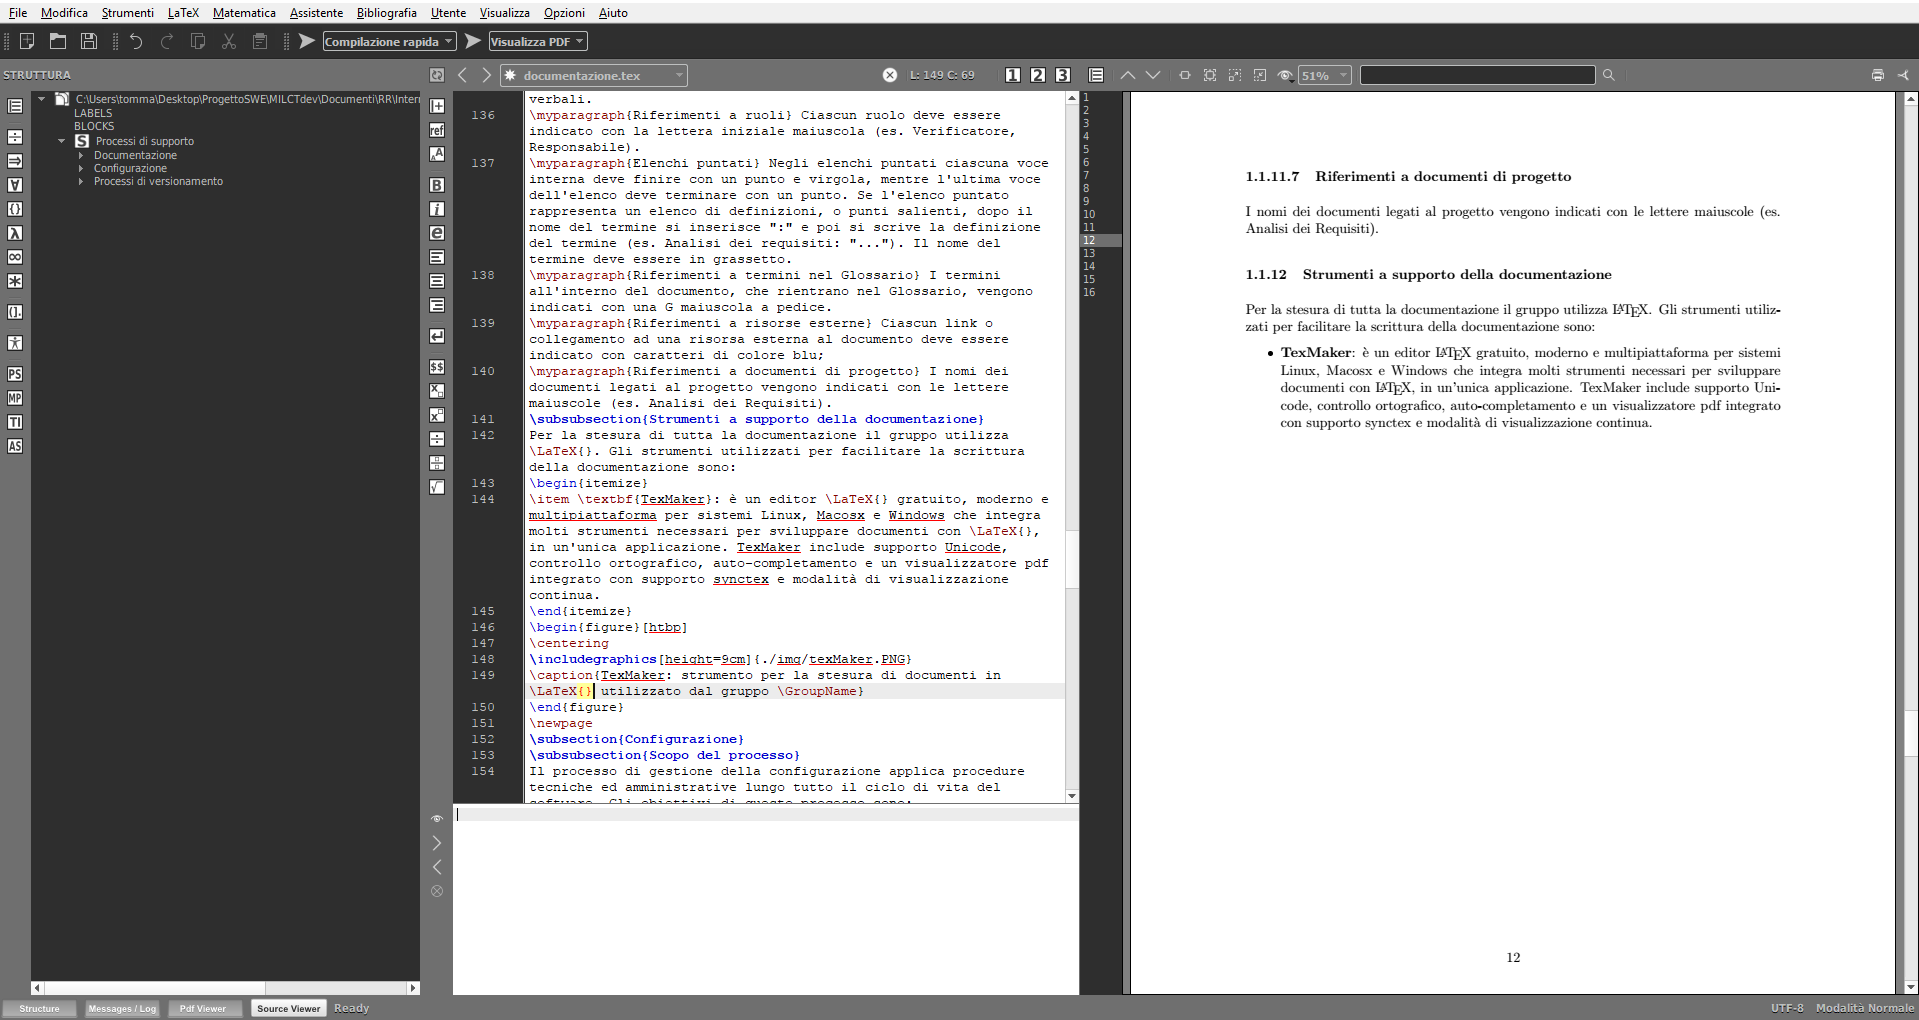
\includegraphics[scale=0.3]{./img/texMaker.png}
						\caption[TexMaker]{TexMaker: editor usato dal gruppo per la stesura di documenti in \LaTeX{}}
					\end{figure}

				\item \textbf{\glossaryItem{Gantt Project}}:
					software gratuito per la creazione di diagrammi di Gantt, rappresentanti task e \glossaryItem{milestone};
				\item \textbf{Microsoft Office Excel 2016}:
					software che permette di creare istogrammi e diagrammi a torta dinamici, in maniera veloce ed intuitiva;
				\item \textbf{Astah}:
					applicazione per la creazione di diagrammi UML di attività;
				\item \textbf{Script per la generazione di tabelle fonti-requisiti}:
					script sviluppato internamente al \glossaryItem{team} in linguaggio PHP per generare il codice \LaTeX{} delle
					tabelle ``fonti-requisiti" e	``requisiti-fonti" presenti in \vAnalisiDeiRequisiti{};
				\item \textbf{Script per l'individuazione di termini di Glossario}:
					script sviluppato dal team in linguaggio PHP che individua, dato un file .tex, tutte le prime occorrenze di termini
					di Glossario in tale file.
			\end{itemize}
